\chapter{Concepts}
\label{chap:concepts}

\section{User Interface}

\begin{figure}
	\caption{\label{fig:firstmockup}A first overview of the screen space distribution}
	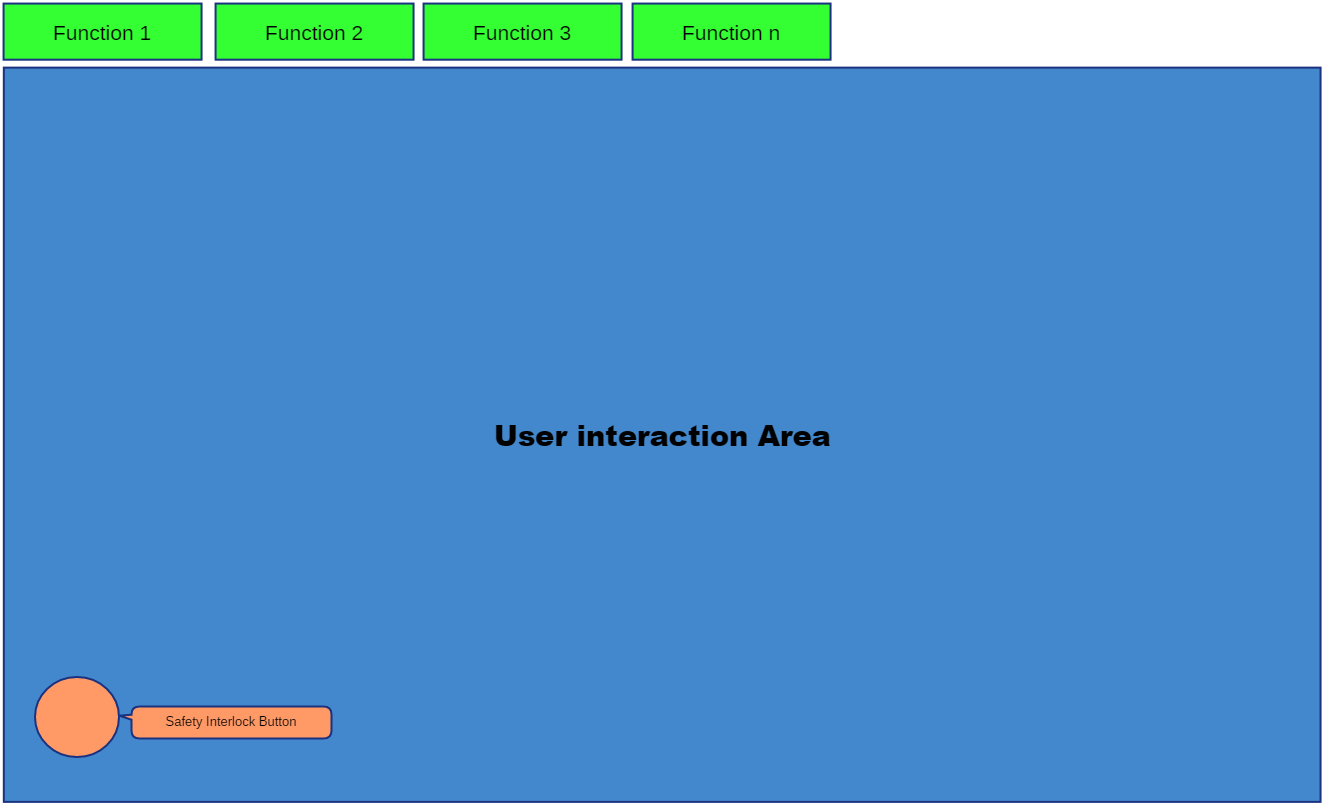
\includegraphics[width=0.9\textwidth]{assets/chpt_concepts/main_touch_interface.png}
\end{figure}

\subsection{Desired position of the Android Tablet}
The application (and thus the screens within it) will be designed for the tablet to be placed in front of the operating person on a table. The person should have clear sight on the controlled robot. It seems sensible to place the tablet on the table in front of the robot while looking at it. Most interactions with the application will be performed by touch gestures using the right hand. For better usability a housing or case can be used to position the tablet at a slight angle to the table. 
% TODO FOTO VOM TABLET AUF TISCH

Interaction with the application is done using the commonly known touch gestures like
\begin{itemize}
	\item Touch (short press on the screen)
	\item Long press (finger remains on a control for a longer period of time)
	\item 1-Finger-Movement
	\item 2-Fingered gestures (\textit{Pinch-Zoom}, Rotation)
	\item 3-Fingered gestures (Rotation, Movement)
\end{itemize}

\subsection{General Screens}

Although a screen with 10 inches diagonal length seems quite big for touch interactions in the first place, it seems even smaller when thinking of the robot interaction space's size and the number of different information that has to be displayed on the screen during control operations of the robot. Since we are mainly operating the robot with touch gestures, significant parts of the screen should be blank, as only few information can be displayed while the user poses his hands above or on the screen. Figure \ref{fig:firstmockup} gives a first overview of how the portions of the screen shall be distributed. The biggest part of the screen is reserved for touch interactions by the user. Since multiple approaches to control the robot shall be implemented, the method shall be selected and switched using a tabbed layout with the tabs on the top, as they then use the least space of the screen.

\subsubsection{Interlock Button}
On all screens where the robot can be remotely operated, a security interlock button shall be displayed. For the actions on the screen to have effect on the robot (i.e. to be sent to the controller) the button shall remain pressed. This implements the functionality of a dead-man-switch, stopping all robot action once released. Although this is only a software measure it should be a good solution against unwanted movements of the robot as the button can easily be released when pressed with a single finger of the left hand.



\section{LWR Robotic Arm Control}
\label{sec:robotarm:ctrl}

\section{Grasp Synergies}

\section{Direct Fingertip Positioning}

\section{Touch Parsing}

\subsection{Grasp Synergies}

\subsection{Direct Fingertip Positioning}

\section{Software Architecture}